\documentclass[letterpaper]{article}
 \usepackage{float}
 \usepackage[margin=2.54cm]{geometry}
 \usepackage{graphicx}
 \usepackage{anysize}
 \usepackage{lipsum}
 \usepackage{amsmath,amssymb,amsthm}
 \usepackage[utf8]{inputenc}
 \usepackage{multirow}
 \usepackage{csquotes}
 \usepackage[spanish]{babel}
 \usepackage{apacite}
 \usepackage{multicol}
 \usepackage{parskip}
 \usepackage{setspace} 
\usepackage{empheq}
\usepackage{mdframed}
\usepackage{booktabs}
\usepackage{lipsum}
\usepackage{graphicx}
\usepackage{color}
\usepackage{psfrag}
\usepackage{pgfplots}
\usepackage{bm}
\usepackage{tocloft}
\geometry{letterpaper, margin=2.54cm}
\begin{document} 
\setstretch{2}
\begin{titlepage}
	\centering
	\vspace{3cm}
	{\scshape\Huge Trabajo de Mecánica de Fluidos \par}
	\vspace{3cm}
	\textbf\large\scshape{\par}
	\vspace{3cm}

	{\Large Vergara Pareja Gustavo\\Pacheco Berrio Jhosuea\\Petro Yanéz Edwin\par}
	\vspace{5cm}
	{\scshape\Large Programa de Ingeniería Mecánica \par}
	{\scshape\Large Universidad de Córdoba\par}
	{\Large \today \par}
\end{titlepage}
\tableofcontents
\newpage
\section{Introducción}
%\%contentsline{toc}{section}{Introducción}
El presente proyecto tiene como objetivo principal aplicar los principios de flotabilidad y estabilidad 
en el diseño y construcción de un bote. La mecánica de fluidos es una rama fundamental de la física que 
estudia el comportamiento de los fluidos en reposo o en movimiento. En este caso, nos enfocaremos en la 
forma en que los fluidos interactúan con el bote y cómo se puede lograr que este flote y se mantenga 
estable en el agua.
\newline

Se responderán preguntas
como: ¿Cómo se diseñó el casco?, ¿Con qué materiales se construyó? y ¿Cuál es su finalidad?.
\newline
Para lograr este objetivo, se utilizarán principios de la física y la mecánica para describir
el movimiento del casco y se analizarán las fuerzas involucradas en su funcionamiento.
Además, se describirá el diseño mecánico de este, incluyendo los materiales utilizados
y las especificaciones técnicas.
\newpage
\section{Objetivos}
%contentsline{toc}{section}{Objetivos}
\subsubsection{Objetivo General}
\begin{itemize}
	\item Diseñar y construir el casco de un bote aplicando los principios de flotabilidad y estabilidad.
\end{itemize}
\subsubsection{Objetivos Específicos}
\begin{itemize}
	\item Analizar y aplicar los conceptos teóricos de la mecánica de fluidos para comprender los principios de flotabilidad y estabilidad en el diseño de embarcaciones.
	\item Diseñar un bote que cumpla con los criterios de flotabilidad y estabilidad, considerando la ubicación del centro de gravedad, el centro de flotación y la forma del casco.
	\item Evaluar experimentalmente el desempeño del bote en términos de flotabilidad y estabilidad, realizando pruebas en condiciones controladas de agua y registrando datos relevantes como la inclinación, el desplazamiento y la capacidad de carga del bote.
\end{itemize}
\newpage

\section{Teoría Relacionada}
%contentsline{toc}{section}{Teoría Relacionada}
\subsubsection{Hidrostática}
\setlength{\parindent}{18pt}

El término hidrostática se refiere al estudio de los fluidos en reposo.

\subsubsection{Fluido}
\setlength{\parindent}{18pt}
Un fluido es una sustancia que se deforma continuamente cuando es sometida 
a un esfuerzo cortante, no importa si el esfuerzo cortante es muy pequeño. (Streter y Wylie, 1997). 

\subsubsection{Principio de Arquímedes}
\setlength{\parindent}{18pt}
Se conoce que los barcos flotan, gracias a los aportes realizados por Arquímedes (Principio de Arquímedes);
la cual establece que, ``La fuerza de flotación que actúa sobre un cuerpo sumergido en un fluido es igual
al peso del fluido desplazado por el cuerpo y actúa hacia arriba pasando por el
centroide del volumen desplazado. Para los cuerpos flotantes, el peso del cuerpo completo debe ser igual a la fuerza
de flotación ($F_{e}$), la cual es el peso del fluido ($W$) cuyo volumen es igual al de la parte sumergida
de ese cuerpo; '', (Cengel and Cimbala, 2020). 
\begin{equation}
	F_{e}= W = \gamma \cdot  V_{sum} 
\end{equation}

\subsubsection{Centro de gravedad}
\setlength{\parindent}{18pt}
Es el punto de aplicación del peso del cuerpo y que no varía con la posición del cuerpo. La ubicación del C.G, 
depende de la forma del objeto, e inclusive pueda que se encuentre fuera del objeto (Hernández et al., 2019).

\subsubsection{Casco de deplazamiento}
\setlength{\parindent}{18pt}
Los barcos con cascos de desplazamiento a menudo se distinguen por una forma de ``V'' profunda en la parte 
inferior o en el casco. Este tipo de casco está diseñado para impulsarse a través del agua, desplazando 
la superficie del agua en una proporción igual al peso de la embarcación (Escola Port Aula Náutica, 2022).
\subsubsection{Dimensiones del Barco}
\setlength{\parindent}{18pt}
Para cualquier diseño de una embarcación que se desea analizar, es necesario conocer cada parte de esta 
estructura ingenieril. Las dimensiones principales que conforman un barco son, eslora máxima, es la longitud 
total del casco, la cual comprende desde la proa hasta la popa, manga máxima, es la mayor anchura de la 
cuaderna con estructuras asentadas, el calado, es la distancia desde la parte inferior de la quilla a la 
línea de flotación, el puntal, es la distancia máxima vertical medida desde la quilla hasta cubierta 
principal, la escora, es el ángulo de inclinación lateral de la embarcación y el asiento, es la diferencia
 en inclinación entre los calados de popa y de proa, esta se clasifica en apopante, apropante y neutro o sentado.
 \begin{figure}[h]
	\centering
	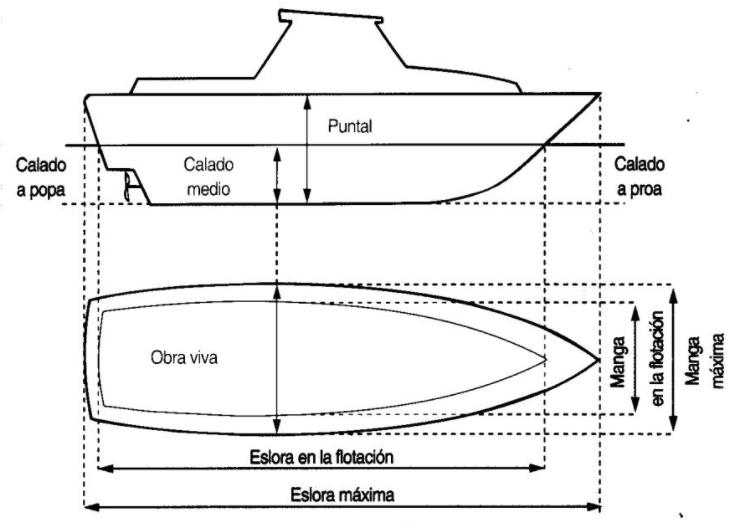
\includegraphics[width=0.5 \textwidth]{dimensionestemporal.jpg}
	\caption{ Dimensiones de un barco}
	\label{fig:imagen00}
\end{figure}
\subsubsection{Estabilidad}
\setlength{\parindent}{18pt}
La estabilidad es la propiedad de un objeto que tiende a volver a su posición original cuando el recipiente 
se mueve fuera del equilibrio uniforme, bajo la influencia de ciertas fuerzas o momentos restauradores. 
En un sistema en movimiento, como un objeto en el agua, la estabilidad a menudo requiere una fuerza de 
restauración y un factor de amortiguamiento (Redín Muñoz, 2007).
\newpage\

\subsubsection{Metacentro}
\setlength{\parindent}{18pt}
El Metacentro, se define como la intercepción del eje vertical de un cuerpo cuando está en su posición 
de equilibrio, con una línea vertical que pasa a través de la nueva posición del centro de flotación 
cuando el cuerpo gira.
\begin{figure}[H]
	\centering
	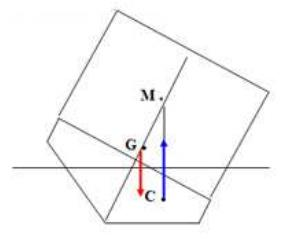
\includegraphics[width=0.3 \textwidth]{Metacentrotemporal.jpg}
	\caption{ Posición del metacentro}
	\label{fig:imagen0}
\end{figure}
Donde:
\newline
\textbf{G}, es el centro de gravedad.
\newline
\textbf{C}, es el centro geométrico de la carena sumergida.
\newline
\textbf{M}, es el punto de cruce de la línea vertical del centro del cuerpo con el plano de la línea central, 
conocido como Metacentro.


Si {M} se sitúa arriba del centro de gravedad, el cuerpo es estable (Mott, 2006).
\subsubsection{Flotabilidad}
\setlength{\parindent}{18pt}
La flotabilidad se define como aquella capacidad que posee un cuerpo para sostenerse dentro de un fluido, 
donde la fuerza flotación actúa en dirección vertical hacia arriba a través del centroide del volumen 
desplazado, (Mott, 2006).
%-
\newpage
\section{¿Qué se hizo?}
%contentsline{toc}{section}{¿Qué se hizo?}
El objetivo de este proyecto fué estudiar el movimiento del casco de un bote y realizar cálculos empíricos
de su flotabilidad, estabilidad y análisis de fuerzas. En la práctica, se construyó el casco de un barco 
a escala y se realizaron experimentos para medir.
\begin{itemize}
	\item El centro de flotabilidad.
	\item El metacentro
	\item
\end{itemize}
\section{Materiales y métodos}
%contentsline{toc}{section}{Materiales y métodos}
Los materiales utilizados para el desarrollo de este casco fueron:
\begin{itemize}
	\item Madera
	\item Pintura
	\item Marcadores
	\item Resina
	\item
	\item
	\item
\end{itemize}

\newpage
\section{Contenido y Resultados}
%contentsline{toc}{section}{Contenido y Resultados}
Para el desarrollo de este proyecto, hicimos una búsqueda exhaustiva de modelos e ideas para construir el casco del barco:
\begin{figure}[H]
	\centering
	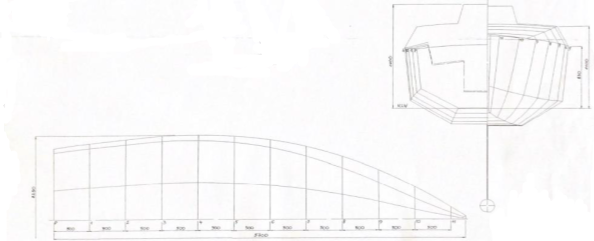
\includegraphics[width=1 \textwidth]{imgbarcoplano.png}
	\caption{ Planos oficiales ClassGlobe 5.80.}
	\label{fig:imagen}
\end{figure}
\begin{itemize}
	\item A continuación, comenzamos a construir el casco del barco.
\end{itemize}
\begin{figure}[H]
	\centering
	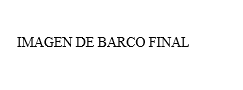
\includegraphics[width=0.5\textwidth]{imgbarcofinal.png}
	\caption{Toma de datos}
	\label{fig:imagen1}
\end{figure}
\begin{itemize}
	\item Luego de esto, pasamos a hacer mediciones y cálculos empíricos:
\end{itemize}
\begin{figure}[H]
	\centering
	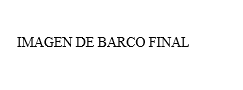
\includegraphics[width=0.8\textwidth]{imgbarcofinal.png}
	\caption{Barco con los criterios solicitados}
	\label{fig:imagen2}
\end{figure}
\begin{itemize}
	\item Análisis del barco
\end{itemize}
\begin{figure}[H]
	\centering
	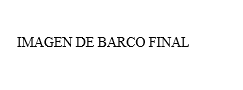
\includegraphics[width=0.8\textwidth]{imgbarcofinal.png}
	\caption{Carga máxima, centro de gravedad y flotabilidad\ldots}
	\label{fig:imagen3}
\end{figure}
\newpage
Con SolidWorks Simulation, es posible realizar análisis de elementos finitos (FEA) para determinar las tensiones, deformaciones y factores de seguridad en la herramienta de corte y otras piezas importantes de la máquina.
Por otro lado, con SolidWorks Motion, es posible simular el movimiento de la máquina y su comportamiento dinámico bajo diferentes condiciones de carga.
\newline
A continuación calcularemos:

\begin{itemize}
	\item Velocidad
	      \newline
	      $$v=\frac{y}{t}=\frac{0.1m}{1s}=10cm/s$$
	\item Aceleracion
	      \newline
	      La aceleración de las cabinas sera igual a 0, ya que por la primera Ley de Newton, estos cuerpos
	      estan bajo velocidad constante.
	\item Tensión
	      \newline
	      Podemos calcular fuerza de tensión en los cables que sostienen las cabinas. Para hacer esto, podemos usar la segunda ley de Newton, que establece que la fuerza neta sobre un objeto es igual a su masa multiplicada por su aceleración. En este caso, la aceleración de las cabinas es cero, por lo que la fuerza neta es cero. Por lo tanto, la suma de las fuerzas en cada cabina debe ser igual a cero. Podemos escribir esto como:
	      \newline
	      $$F_{T}-\left ( m_{1}*g \right )-\left ( m_{2}*g \right )=0$$
	      $$F_{T}=\left ( 0.04kg*9.81\frac{m}{{s}^2} \right )+\left ( 0.04kg*9.81\frac{m}{{s}^2} \right )=0.8N$$
	\item Potencia
	      $$W=2T\cdot v=\left ( 0.8N \right )\left ( 0.1m/s \right )=0.08W$$
	\item Velocidad angular del eje:
	      \newline
	      Podemos calcular la velocidad angular del eje utilizando la fórmula:
	      \newline
	      $$w = v/r$$
	      $$w =\left ( 0.1m/s \right )/\left ( 0.02m \right )=5 rad/s$$
\end{itemize}
\section{Conclusiones}
%contentsline{toc}{section}{Conclusiones}
En conclusión, el proyecto de diseño y construcción de un bote basado en los principios de flotabilidad y estabilidad es una oportunidad para aplicar los conocimientos teóricos de la mecánica de fluidos de manera práctica y significativa. A lo largo del proyecto, se han abordado conceptos clave como el principio de Arquímedes, el centro de flotación, la estabilidad y la resistencia hidrodinámica.
El diseño y construcción de un bote que cumpla con los principios mencionados requiere un enfoque integral que considere tanto los aspectos teóricos como los prácticos. Se han explorado conceptos teóricos fundamentales y se han aplicado en la práctica a través de la construcción del bote y la evaluación experimental de su desempeño en términos de flotabilidad y estabilidad.
Este proyecto ha permitido comprender la relación entre la teoría de la mecánica de fluidos y su aplicación práctica en el diseño y construcción de embarcaciones. Estos conocimientos adquiridos son valiosos tanto en el ámbito académico como en el profesional, ya que la mecánica de fluidos juega un papel fundamental en numerosas disciplinas relacionadas con el diseño


\newpage
\section*{}
\bibliographystyle{apacite}
\nocite{*}
\bibliography{referenciados}
\end{document}